\documentclass[tikz]{standalone}

\begin{document}
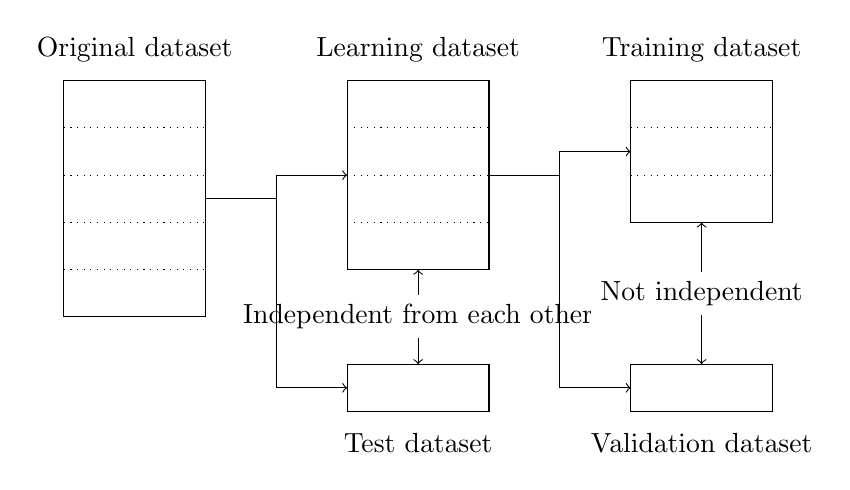
\begin{tikzpicture}[scale=0.1]


% 元データ
\draw (0,18) rectangle (18,48);
\node[] at (9,52) {Original dataset};

% 学習データ
\draw (36,24) rectangle (54,48);
\node[] at (45,52) {Learning dataset};

% テストデータ
\draw (36,6) rectangle (54,12);
\node[] at (45,2) {Test dataset};

% トレーニングデータ
\draw (72,30) rectangle (90,48);
\node[] at (81,52) {Training dataset};

% バリデーションデータ
\draw (72,6) rectangle (90,12);
\node[] at (81,2) {Validation dataset};

% 学習--テスト
\draw[<->] (45,12)--(45,24);
\node[fill=white] at (45,18) {Independent from each other};

% トレーニング--バリデーション
\draw[<->] (81,12)--(81,30);
\node[fill=white] at (81,21) {Not independent};

% 1--2カラム
\draw[->](18,33)--(27,33)--(27,36)--(36,36);
\draw[->](27,33)--(27,9)--(36,9);

% 2--3カラム
\draw[->](54,36)--(63,36)--(63,39)--(72,39);
\draw[->](63,36)--(63,9)--(72,9);

% 点線
\draw[dotted] (0,24)--(18,24);
\draw[dotted] (0,30)--(18,30);
\draw[dotted] (0,36)--(18,36);
\draw[dotted] (0,42)--(18,42);

\draw[dotted] (36,30)--(54,30);
\draw[dotted] (36,36)--(54,36);
\draw[dotted] (36,42)--(54,42);

\draw[dotted] (72,36)--(90,36);
\draw[dotted] (72,42)--(90,42);




\end{tikzpicture}
\end{document}